\documentclass[15pt,a5paper,reqno]{article}
\usepackage{hyperref}
\usepackage[warn]{mathtext}
\usepackage[utf8x]{inputenc}
\usepackage{amssymb, amsmath, multicol}
\usepackage[russian]{babel}
\usepackage{graphicx}
\usepackage[shortcuts,cyremdash]{extdash}
\usepackage{wrapfig}
\usepackage{floatflt}
\usepackage{lipsum}
\usepackage{verbatim}
\usepackage{concmath}
\usepackage{euler}
\usepackage{xcolor}
\usepackage{etoolbox}
\usepackage{fancyhdr}
\usepackage{subfiles}
\usepackage{enumitem}
\usepackage{amsthm}
\usepackage{indentfirst}
\usepackage{import}

\DeclareMathOperator{\sign}{sign}

\RequirePackage[ left     = 1.5cm,
  right    = 1.5cm,
  top      = 2.0cm,
  bottom   = 1.25cm,
  includefoot,
  footskip = 1.25cm ]{geometry}
\setlength    {\parskip}        { .5em plus .15em minus .08em }
%\setlength    {\parindent}      { .0em }
\renewcommand {\baselinestretch}{ 1.07 }

\fancyhf{}

\renewcommand{\footrulewidth}{ .0em }
\fancyfoot[C]{\texttt{\textemdash~\thepage~\textemdash}}
\fancyhead[R]{\hfilШурыгин}

\makeatletter
\patchcmd\l@section{%
  \nobreak\hfil\nobreak
}{%
  \nobreak
  \leaders\hbox{%
    $\m@th \mkern \@dotsep mu\hbox{.}\mkern \@dotsep mu$%
  }%
  \hfill
  \nobreak
}{}{\errmessage{\noexpand\l@section could not be patched}}
\makeatother
\parindent = 1cm % отступ при красной строке⏎
\pagestyle{fancy}    
\renewcommand\qedsymbol{$\blacksquare$}

\newcommand{\when}[2]{
  \left. #1 \right|_{#2} \hspace
}
\renewcommand{\kappa}{\varkappa}
\RequirePackage{caption2}
\renewcommand\captionlabeldelim{}
\newcommand*{\hm}[1]{#1\nobreak\discretionary{}

\DeclareSymbolFont{T2Aletters}{T2A}{cmr}{m}{it}
{\hbox{$\mathsurround=0pt #1$}}{}}
% Цвета для гиперссылок
\definecolor{linkcolor}{HTML}{000000} % цвет ссылок
\definecolor{urlcolor}{HTML}{799B03} % цвет гиперссылок
 
\hypersetup{pdfstartview=FitH,  linkcolor=linkcolor,urlcolor=urlcolor, colorlinks=true}


%\setcounter{secnum[utf8x]depth}{0}

\begin{document}

% НАЧАЛО ТИТУЛЬНОГО ЛИСТА
\begin{center}
  {\small ФЕДЕРАЛЬНОЕ ГОСУДАРСТВЕННОЕ АВТОНОМНОЕ ОБРАЗОВАТЕЛЬНОЕ\\ УЧРЕЖДЕНИЕ ВЫСШЕГО ОБРАЗОВАНИЯ\\ МОСКОВСКИЙ ФИЗИКО-ТЕХНИЧЕСКИЙ ИНСТИТУТ\\ (НАЦИОНАЛЬНЫЙ ИССЛЕДОВАТЕЛЬСКИЙ УНИВЕРСИТЕТ)\\ ФИЗТЕХ-ШКОЛА РАДИОТЕХНИКИ И КИБЕРНЕТИКИ}\\
  \hfill \break
  \hfill \break
  \hfill \break
  \Huge{Дифракция света на периодических структурах (саморепродукция).}\\
\end{center}

\hfill \break
\hfill \break
\hfill \break
\hfill \break
\hfill \break
\hfill \break

\begin{flushright}
  \normalsize{Работу выполнил:}\\
  \normalsize{\textbf{Шурыгин Антон Алексеевич, группа Б01-909}}\\
\end{flushright}

\begin{center}
  \normalsize{\textbf{Долгопрудный, 2021}}
\end{center}


\thispagestyle{empty} % выключаем отображение номера для этой страницы

% КОНЕЦ ТИТУЛЬНОГО ЛИСТА

\newpage
\thispagestyle{plain}
\tableofcontents
\thispagestyle{plain}
\newpage


\textbf{Цель работы:}
Изучение явления саморепродукции и применение его к измерению параметров периодических структур.

\textbf{Оборудование:} лазер,кассета с сетками, мира, короткофокусная линза с микрометрическим винтом, экран, линейка.

\section{Введение и краткая теория}
При дифракции на предмете с периодической структурой наблюдается явление саморепродукции: на некотором расстоянии от предмета вдоль направления распространения волны появляется изображение, которое потом периодически повторяется.  \par
Представим волну за периодическим объектом в виде суммы плоских волн разных направлений. Отдельные слагаемые плоские волны называют пространственными гармониками. Вдоль пути распространения волнового фронта на некотором расстоянии $z_0$ от предмета существует плоскость, где разность фазовых набегов любых пространственных гармоник (плоских волн идущих под углом $\theta$т к оси распространения), входящих в состав суперпозиции, кратна $2T$ В этой плоскости фазовые соотношения между всеми плоскими волнами, входящими в состав суперпозиции, такие же, что и в предметной плоскости. Поэтому в результате интерференции этих волн возникает изображение, тождественное исходному периодическому объекту. Все сказанное справедливо для любого расстояния $z_n$, кратного $z_0$. Для решетки с периодом $d$.
\begin{equation}
    z_n = \frac{2d^2}{\lambda}n
\end{equation}

Суть эксперимента по саморепродукции состоит в том, что дифрагированная на периодическом транспаранте (решетка, сетка) плоская монохроматическая волна лазера (лазерный пучок) воспроизводит изображение транспаранта без каких-либо оптических элементов.

    \begin{figure}[h]
    \centering
    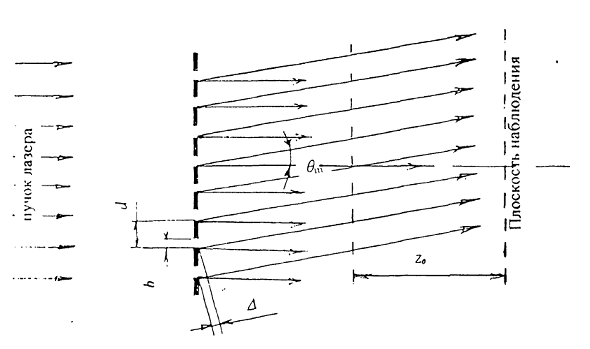
\includegraphics[width=15cm]{pics/fig1.png}
    \caption{Дифракция лучей на сетке и возникновение саморепродуцированного изображения}
    \label{fig:vac}
\end{figure}

\section{Схема установки}

    \begin{figure}[h]
    \centering
    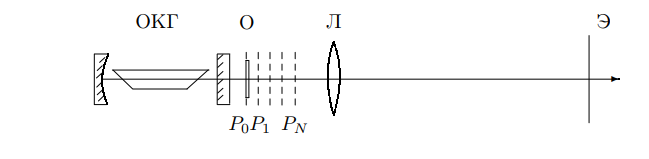
\includegraphics[width=15cm]{pics/scheme.png}
    \caption{Схема лабораторной установки}
    \label{fig:vac}
\end{figure}

\section{Ход работы}

\end{document}